

Let us zoom in a little on the previous graphes: 


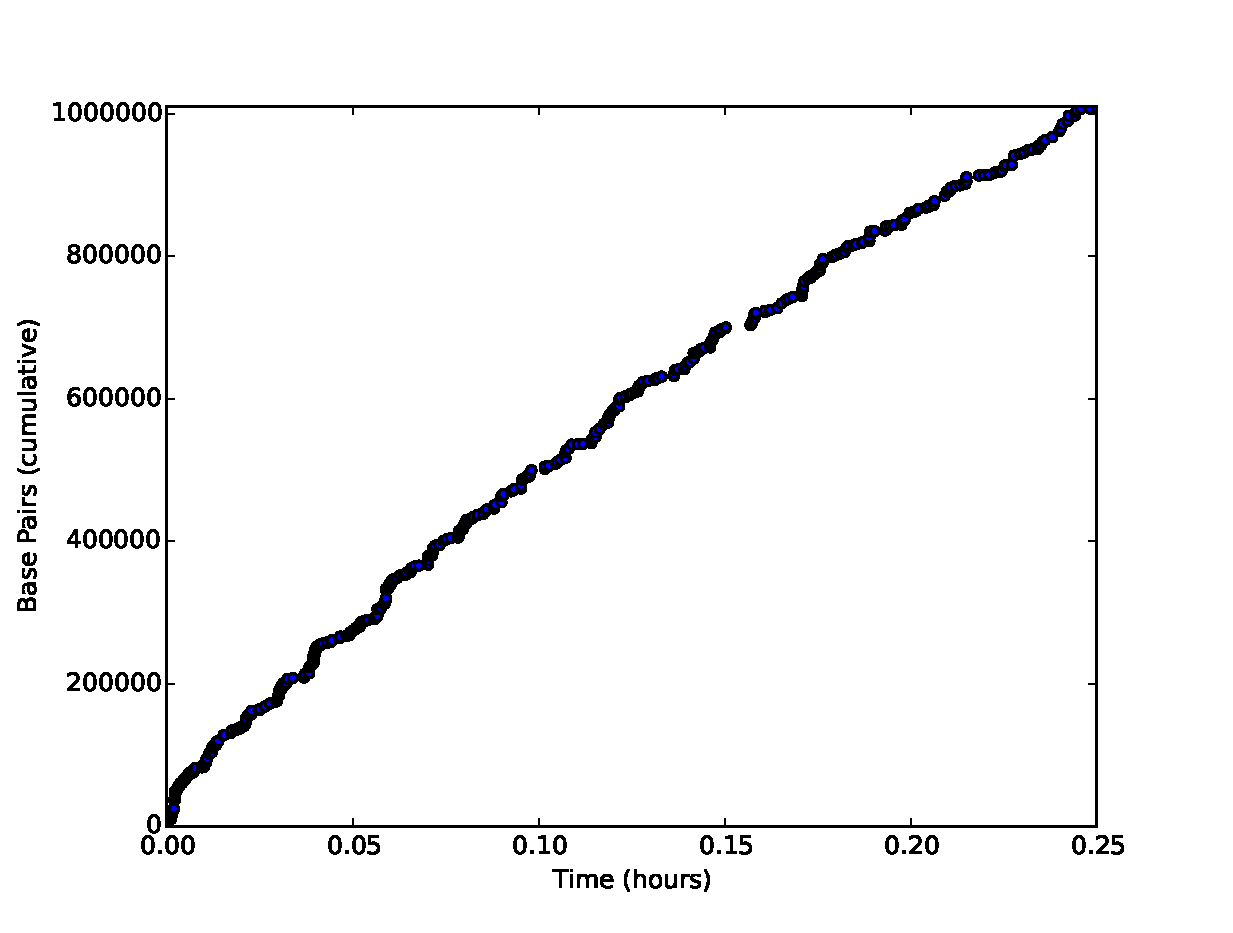
\includegraphics[width=0.48\textwidth]{q4qh}
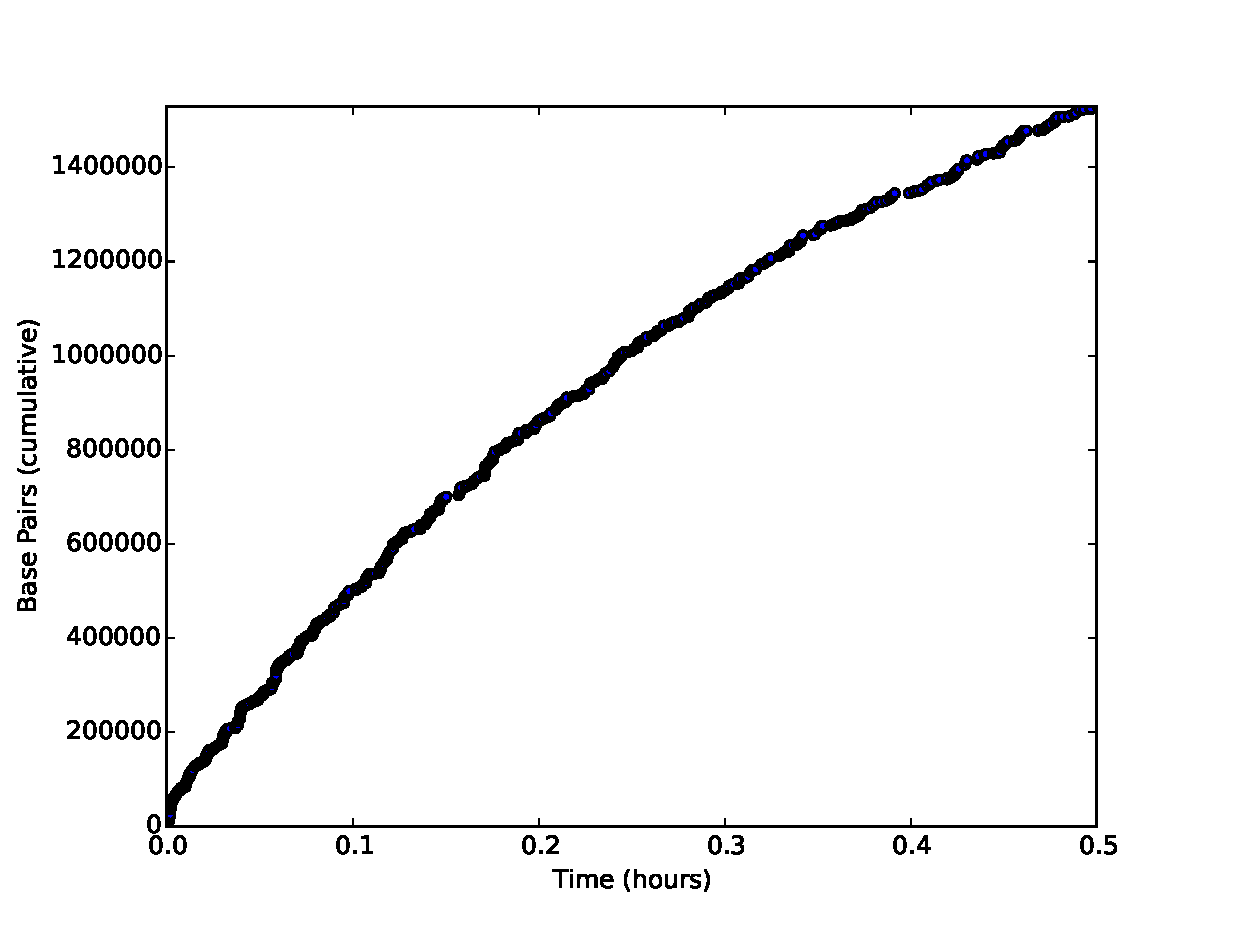
\includegraphics[width=0.48\textwidth]{q4hh}

The first quarter hour appears linear, but the first half hour does not.

To estimate the amout of time needed to sequence the human genome once, 
we used data from the first quarter hour due to its linearity.  We hypothesize 
that the change in sequencing rate is due to a decrease in the molar concentration 
of DNA, and therefore the rate at which a DNA molecule encounters a given pore is 
rate-limiting, rather than a decrease in the effeciecy of the MinION.  Therefore, 
in our calculation, we made the assumption that DNA concentration does not change 
over time and there is only one copy of the genome present to avoid sequencing 
$>$ 1x coverage. 

